\paragraph{QuizziPedia::Back-End::App::Controllers::UserController}
\label{QuizziPedia::Back-End::App::Controllers::UserController}
\begin{figure}
	\centering
	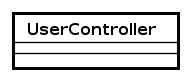
\includegraphics[scale=0.45]{UML/Classi/Back-End/QuizziPedia_Back-End_App_Controllers_UserController.png}
	\caption{QuizziPedia::Back-End::App::Controllers::UserController}
\end{figure}
\FloatBarrier
\begin{itemize}
	\item 
	\textbf{Descrizione}:\\
	Classe che raggruppa attraverso require i vari controllers responsabili delle operazioni legate alla gestione degli utenti. Si è scelto di predisporre questo raggruppamento per facilitare l'introduzione di nuove funzionalità legate alla gestione degli utenti.
	\item \textbf{Utilizzo}:\\
	Viene utilizzata per raggruppare i controllers responsabili della gestione dei dati degli utenti. In questo modo le classi che vogliono comunicare con i controllers legati agli utenti necessitano di includere solo questa classe e non ogni singolo controller.
	\item \textbf{Relazioni con altre classi}:\\
	\begin{itemize}
		\item 
			IN	\texttt{UserRouter}\\
			Classe che gestisce le richieste relative alla registrazione e alla gestione della sessione di un utente. Componente ConcreteHandler del design pattern Chain of responsibility. Utilizza il modulo Passport.		
		\item 
			OUT \texttt{SessionController}\\
			Classe middleware che, utilizzando Passport, si occupa di controllare la consistenza dell'oggetto session durante la sessione associata all'utente autenticato. È un componente ConcreteHandler del design pattern Chain of responsibility.
		\item 
			OUT \texttt{AuthenticationController}\\
			Classe che si occupa della registrazione e dell'autenticazione dell'utente nel sistema. È un componente ConcreteHandler del design pattern Chain of responsibility. Risulta essere il componente che eventualmente esegue la richiesta del client attraverso Passport.	
		\item 
			OUT \texttt{UserManagementController}\\
			Classe che gestisce la logica applicativa riguardante la visualizzazione e la modifica dei dati dell'utente.
			Rappresenta il ConcreteHandler nel design pattern Chain of responsibility. Utilizza Passport.
	\end{itemize}
\end{itemize}
